\pdfobjcompresslevel=0
%\pdfminorversion=5

%\documentclass[xcolor=dvipsnames, 8pt, aspectratio=149]{beamer}
\documentclass{beamer} 

\usetheme{progressbar}
\setbeamertemplate{footline}[frame number]
\setbeamercovered{transparent}
\useinnertheme{default}

%\usepackage[francais]{babel}
\usepackage[utf8]{inputenc}
\usepackage[T1]{fontenc}
\usepackage[english]{babel}
%\usepackage[latin1]{inputenc}
%\usepackage[latin1]{inputenc}


\usepackage{tikz}
\usepackage{graphicx}
\graphicspath{{img/}}
\DeclareGraphicsExtensions{.pdf,.jpeg,.png,.eps}
\usepackage{amsmath}
\usepackage{amsfonts}
\usepackage{amssymb}
\usepackage{dsfont}

\usepackage{subfigure}
\usepackage{rotating}

\usepackage{array}
\newcolumntype{M}[1]{>{\raggedright}m{#1}}
\usepackage{multirow}

\usepackage{ragged2e} 
\usepackage{lipsum} 
\usepackage{fourier-orns}
\usepackage{dirtytalk}
\usepackage{color}

\usepackage[plain]{algorithm}
\usepackage{algorithmic}

\DeclareMathOperator*{\argmin}{\arg\!\min}

\definecolor{dgreen}{rgb}{0.,0.6,0.}
\definecolor{azure}{rgb}{0.,0.5,1.}
\definecolor{bluegray}{rgb}{0.4,0.6,0.8}
\definecolor{bleu}{rgb}{0.19,0.55,0.91}
\definecolor{gray}{rgb}{0.75,0.75,0.75}

\newtheorem{prop}{Property}
\newtheorem{thm}{Theorem}
\newtheorem{rem}{Remark}


\def\todo{\color{green}}


\title{Unsupervised anomaly detection}
\author{Albert Thomas - PhD Student\\
		Airbus Group Innovations - Telecom ParisTech \\
		\footnotesize Supervisors: Vincent Feuillard (Airbus), Stéphan Clémençon (Telecom) and Alexandre Gramfort (Telecom)
		}
\date{September 28th, 2016}


\begin{document}

\begin{frame}\frametitle{Unsupervised anomaly detection}
Data set: $X_1, \dots, X_n \in \mathbb{R}^d$ ($d =$ number of parameters)
\begin{itemize}
	\item Unlabeled data set.
	\item Anomaly $=$ rare
\end{itemize}


Statistical approach
\begin{itemize}
	\item $X_1, \dots, X_n$ realizations of an unknown probability distribution $P$
	\item $\lambda$ Lebesgue measure
	\item Find the normal region: region of minimum volume among all regions with probability greater than $\alpha \in (0,1)$
\end{itemize}

\begin{minipage}{0.55\textwidth}
	\begin{center}
	\textbf{Minimum volume set} {\color{bleu}[Polonik, 1997]}
	\end{center}
	\begin{equation*}
	\Omega^*_{\alpha} = \argmin_{\Omega \in \mathcal{B}(\mathbb{R}^d)} \{\lambda(\Omega), P(\Omega) \geq \alpha \}
	\end{equation*}

	\begin{center}
	(density level set with regularity assumptions)
	\end{center}
\end{minipage}
\begin{minipage}{0.35\textwidth}
	\centering
	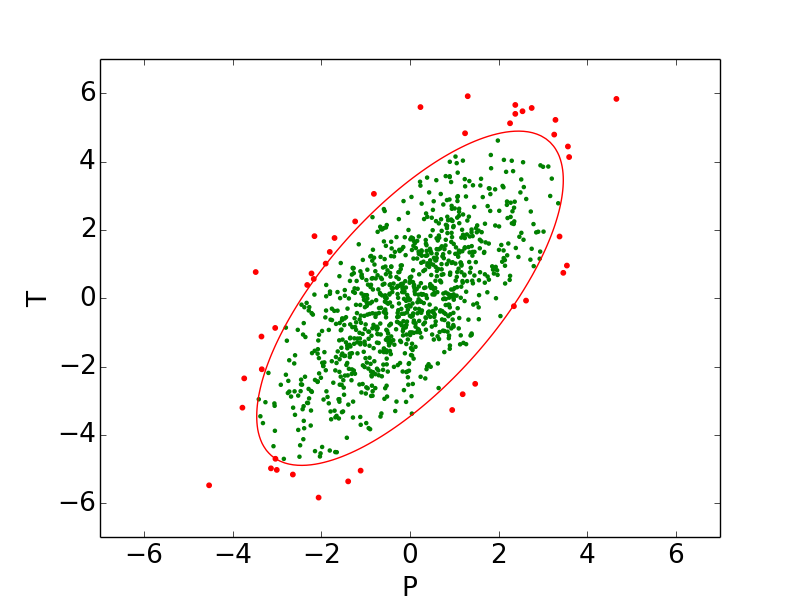
\includegraphics[width=0.95\textwidth]{img/anomaly_detection_end_col.png}
\end{minipage}


\end{frame}



\begin{frame}\frametitle{Mass Volume curve}

\textbf{Mass Volume curve} $\text{MV}_s$ of a scoring function $s$ {\color{bleu}[Clémençon and Jakubowicz, 2013]}:
\begin{equation*}
t \in \mathbb{R} \mapsto (\alpha_s(t), \lambda_s(t))
\end{equation*}
\begin{itemize}
\item $\alpha_s(t) = \mathbb{P}(s(X) \geq t)$ \textbf{mass}
\vspace{0.2cm}
\item $\lambda_s(t) = \lambda(\{x, s(x) \geq t\})$ \textbf{volume}
\end{itemize}

\begin{figure}[htb]
\centering
\subfigure[Scoring functions]{%
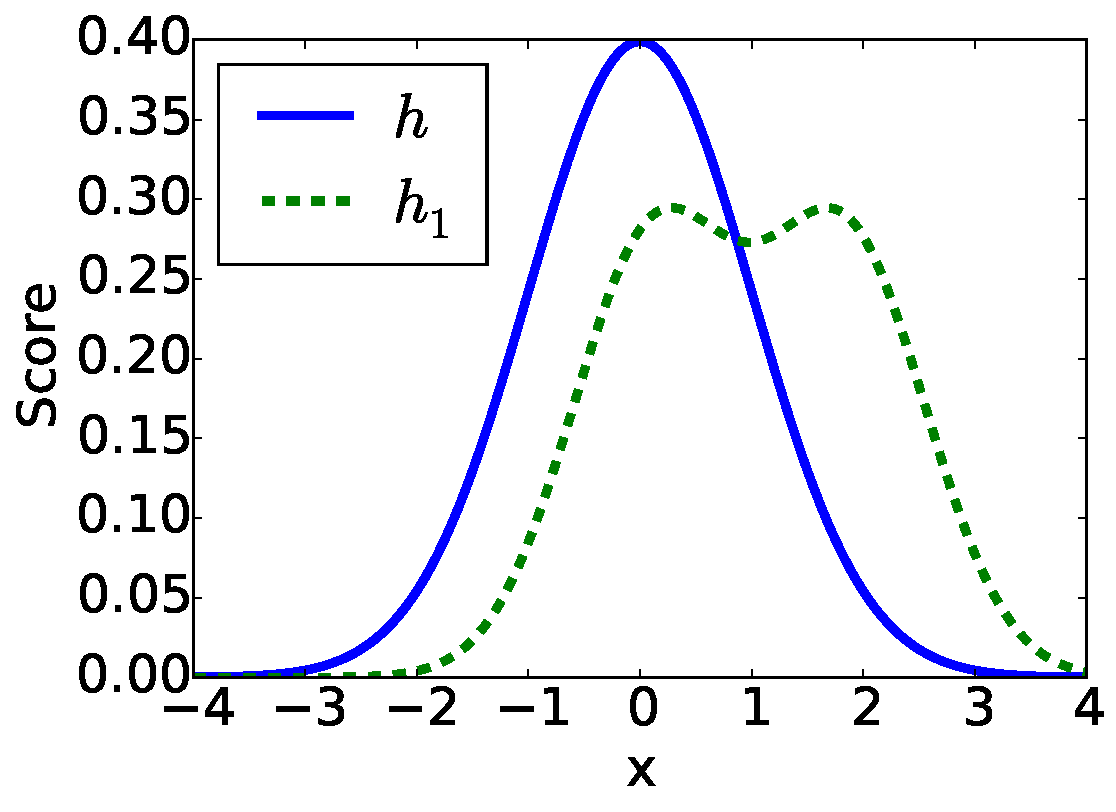
\includegraphics[width=0.45\columnwidth]{mv_curves_examples_1_comp.pdf}}
\subfigure[Mass Volume curves]{%
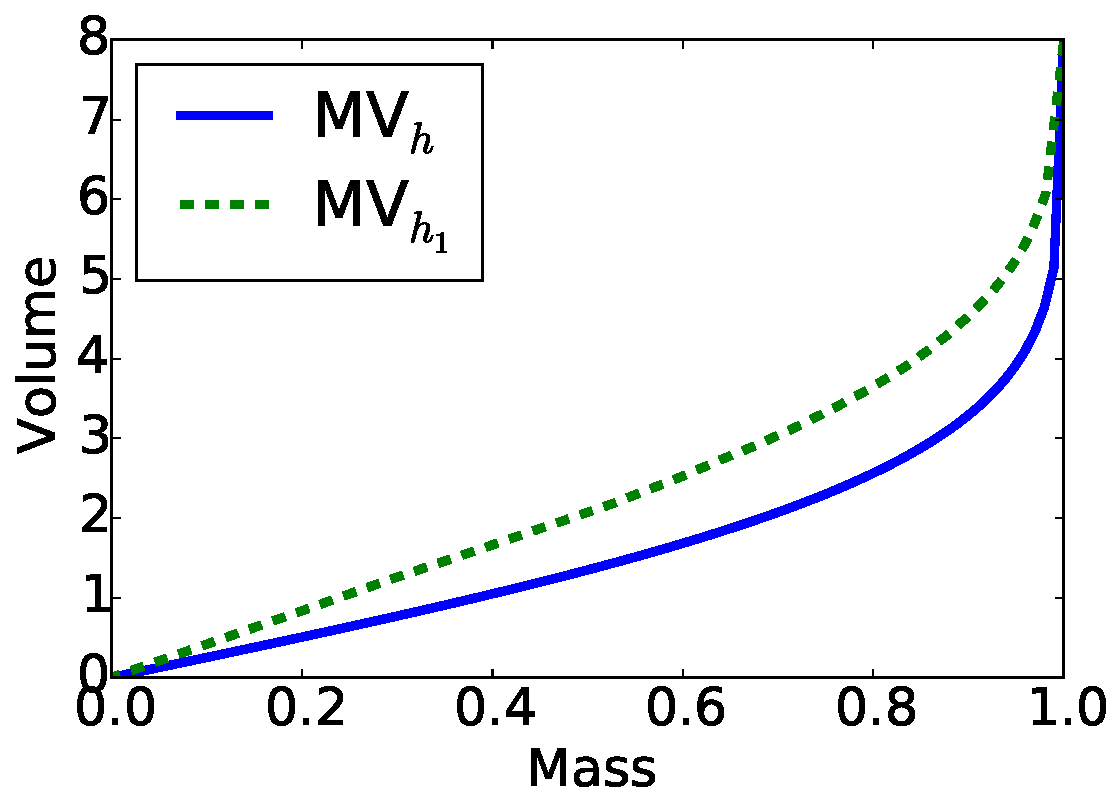
\includegraphics[width=0.45\columnwidth]{mv_curves_examples_2_comp.pdf}}
\end{figure}


\end{frame}


\begin{frame}\frametitle{Mass Volume curve}

\vspace{-0.8cm}

$\text{MV}_s$ also defined as the plot of the function
\begin{equation*}
\text{MV}_s : \alpha \in (0, 1) \mapsto \lambda_s(\alpha_s^{-1}(\alpha)) = \lambda(\{x, s(x) \geq \alpha_s^{-1}(\alpha)\})
\end{equation*}
where $\alpha_s^{-1}$ generalized inverse of $\alpha_s$.

\vspace{0.2cm}
\begin{block}{Property {\color{bleu}[Clémençon and Jakubowicz, 2013]}}
Assume that the underlying density $h$ has no flat parts. Let $\text{MV}^*$ be the MV curve of $h$, then for all scoring functions $s$,
\begin{equation*}
\forall \alpha \in (0, 1), \quad \text{MV}^*(\alpha) \leq \text{MV}_s(\alpha) \enspace
\end{equation*}
\end{block}

\centering \textbf{The closer is $\text{MV}_s$ to $\text{MV}^*$ the better is $s$}


\end{frame}



\end{document}

